\documentclass[12pt, a4paper]{article}

\usepackage[utf8]{inputenc}
\usepackage[T1]{fontenc}
\usepackage{geometry}
\geometry{a4paper, top=25mm, bottom=25mm, left=25mm, right=25mm}
\usepackage{graphicx}
\usepackage{amsmath, amssymb}
\usepackage{booktabs}
\usepackage{float}
\usepackage{caption}
\usepackage{subcaption}
\usepackage{xcolor}
\usepackage{textcomp}
\usepackage{hyperref}
\usepackage{listings}
\usepackage{enumitem}
\usepackage{tikz}
\usetikzlibrary{shapes.geometric, arrows, positioning}

% ===== TikZ Flowchart Styles =====
\tikzstyle{startstop} = [rectangle, rounded corners, minimum width=3cm, minimum height=1cm,text centered, draw=black, fill=red!30]
\tikzstyle{io} = [trapezium, trapezium left angle=70, trapezium right angle=110, minimum width=3cm, minimum height=1cm, text centered, draw=black, fill=blue!30]
\tikzstyle{process} = [rectangle, minimum width=3cm, minimum height=1cm, text centered, draw=black, fill=orange!30]
\tikzstyle{decision} = [diamond, minimum width=3cm, minimum height=1cm, text centered, draw=black, fill=green!30]
\tikzstyle{arrow} = [thick,->,>=stealth]

% ===== Code Listing Settings =====
\definecolor{codegreen}{rgb}{0,0.6,0}
\definecolor{codegray}{rgb}{0.5,0.5,0.5}
\definecolor{codepurple}{rgb}{0.58,0,0.82}
\definecolor{backcolour}{rgb}{0.95,0.95,0.92}

\lstdefinestyle{mystyle}{
    backgroundcolor=\color{backcolour},   
    commentstyle=\color{codegreen},
    keywordstyle=\color{magenta},
    numberstyle=\tiny\color{codegray},
    stringstyle=\color{codepurple},
    basicstyle=\ttfamily\footnotesize,
    breakatwhitespace=false,         
    breaklines=true,                 
    captionpos=b,                    
    keepspaces=true,                 
    numbers=left,                    
    numbersep=5pt,                  
    showspaces=false,                
    showstringspaces=false,
    showtabs=false,                  
    tabsize=2,
    literate={∠}{{$\angle$}}1 {°}{{$^\circ$}}1
}
\lstset{style=mystyle}

% ===== Plot path =====
\graphicspath{{images/}}

\begin{document}

\begin{titlepage}
    \vspace*{\fill}
    \centering
    {\Huge \textbf{Analysis of Synchronous Generator Control, Parallel Operation, and Grid Synchronization}\par}
    \vspace{1.5cm}
    {\Large \textbf{Project Report}\par}
    \vspace{2cm}
    {\Large \textbf{Author:}\par}
    {\Large PERERA J.D.T.\par}
    \vspace{0.5cm}
    {\Large \textbf{Student ID:}\par}
    {\Large E/21/291\par}
    \vspace{0.5cm}
    {\Large \textbf{Date:}\par}
    {\Large \today\par}
    
    \vspace*{\fill}
    
    \begin{center}
        \textbf{Course:} EE-354 Power Engineering \\
        \textbf{Assignment:} Assignment 1 -- Synchronous Generators
    \end{center}
\end{titlepage}

% ===== Table of Contents =====
\tableofcontents
\newpage

% ===== Nomenclature =====
\section*{Nomenclature}
\addcontentsline{toc}{section}{Nomenclature}
\begin{table}[H]
    \centering
    \begin{tabular}{llp{10cm}}
        \toprule
        \textbf{Symbol} & \textbf{Unit} & \textbf{Description} \\
        \midrule
        $E_a$, $E_B$ & pu / V & Internal generated voltage (EMF) of a synchronous machine \\
        $V_t$, $V_{\text{bus}}$ & pu / V & Terminal voltage \\
        $P$, $Q$ & pu / W, VAr & Active and reactive power \\
        $f$, $\omega$ & Hz, rad/s & Electrical frequency and angular velocity \\
        $\delta$ & rad / deg & Rotor load angle (power angle) \\
        $H$ & s & Inertia constant \\
        $R$ & pu & Governor speed droop \\
        $X_d$, $X_q$ & pu & Direct and quadrature axis synchronous reactances \\
        $K_a$, $T_a$ & -- , s & Automatic Voltage Regulator (AVR) gain and time constant \\
        \bottomrule
    \end{tabular}
\end{table}
\newpage

% ========================================================================
%                           EXERCISE 1
% ========================================================================
\section{Exercise 1: Synchronous Machine Control}

This exercise examines the behavior of a single synchronous machine connected to a load, based on the MATLAB Simulink example \texttt{SMControlExample}. The model was copied locally and run without modifications.

\subsection{Simulation Model}

\begin{figure}[H]
    \centering
    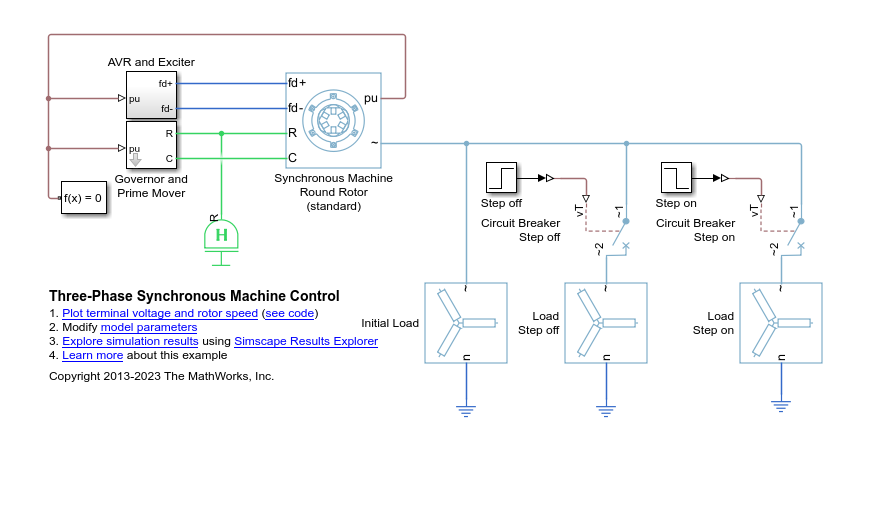
\includegraphics[width=\textwidth]{EX1_diagram.png}
    \caption{Simulink model for Exercise 1 -- Single synchronous machine connected to a load.}
    \label{fig:ex1_model}
\end{figure}

% ----- Task 1 -----
\subsection{Task 1: Component Analysis}

\subsubsection{Synchronous Machine}

The synchronous machine is the core electromechanical energy conversion device. In the Simulink model, it is represented by a detailed d-q axis model capturing both electrical dynamics (stator and rotor windings) and mechanical dynamics (rotor inertia).

\begin{figure}[H]
    \centering
    \begin{subfigure}[b]{0.48\textwidth}
        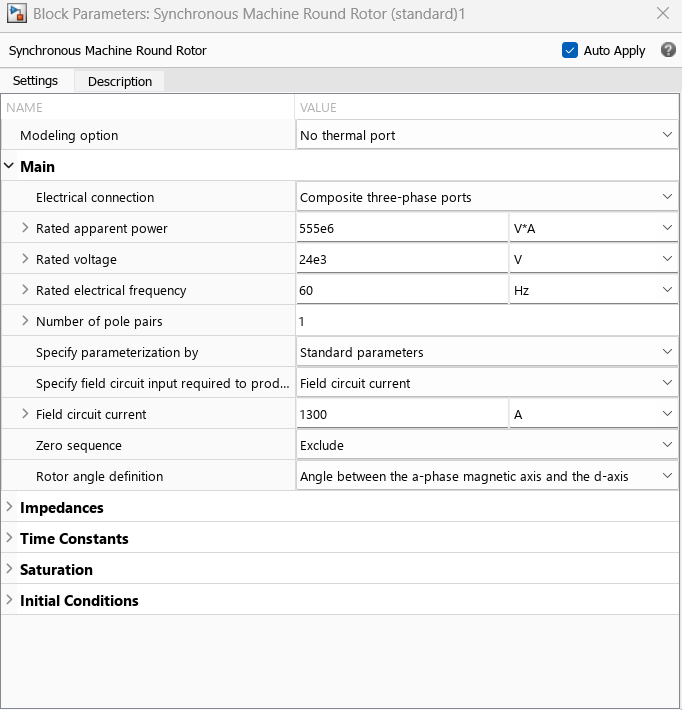
\includegraphics[width=\textwidth]{SYNC_GEN_parameters_main.png}
        \caption{Main parameters}
    \end{subfigure}
    \hfill
    \begin{subfigure}[b]{0.48\textwidth}
        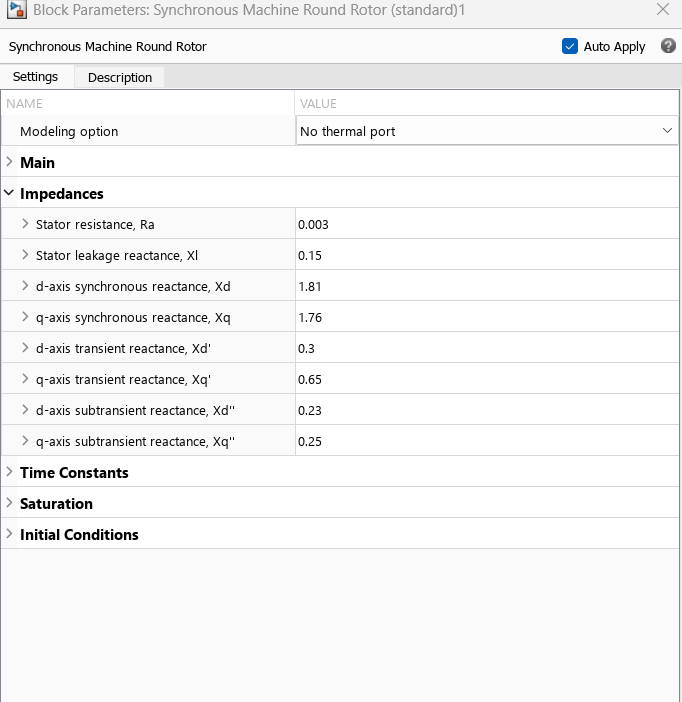
\includegraphics[width=\textwidth]{SYNC_GEN_parameters_impedances.png}
        \caption{Impedance parameters}
    \end{subfigure}
    \\[0.5cm]
    \begin{subfigure}[b]{0.48\textwidth}
        \centering
        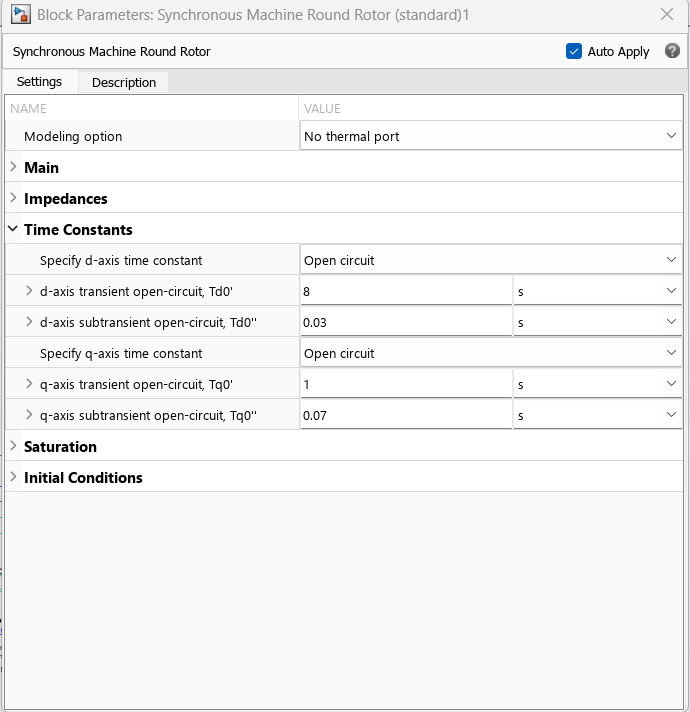
\includegraphics[width=\textwidth]{SYNC_GEN_parameters_timeconstants.png}
        \caption{Time constants}
    \end{subfigure}
    \caption{Synchronous machine block parameters from the Simulink model.}
    \label{fig:sync_gen_params}
\end{figure}

\textbf{Governing Equations:}

The internal generated voltage:
\begin{equation}
    E_a = K \cdot \phi \cdot \omega = K \cdot I_f \cdot \omega
    \label{eq:emf}
\end{equation}

The terminal voltage in phasor form:
\begin{equation}
    \vec{V}_t = \vec{E}_a - j X_d \vec{I}_d - j X_q \vec{I}_q - R_s \vec{I}_a
    \label{eq:terminal_voltage}
\end{equation}

The power-angle relationship:
\begin{equation}
    P = \frac{E_a V_t}{X_d} \sin\delta + \frac{V_t^2 (X_d - X_q)}{2 X_d X_q} \sin 2\delta
    \label{eq:power_angle}
\end{equation}

\subsubsection{Automatic Voltage Regulator (AVR) and Exciter}

The AVR maintains the terminal voltage $V_t$ at a desired reference value $V_{\text{ref}}$. It continuously senses $V_t$, compares it with $V_{\text{ref}}$, and adjusts the field voltage $E_{fd}$ through the exciter.

\begin{figure}[H]
    \centering
    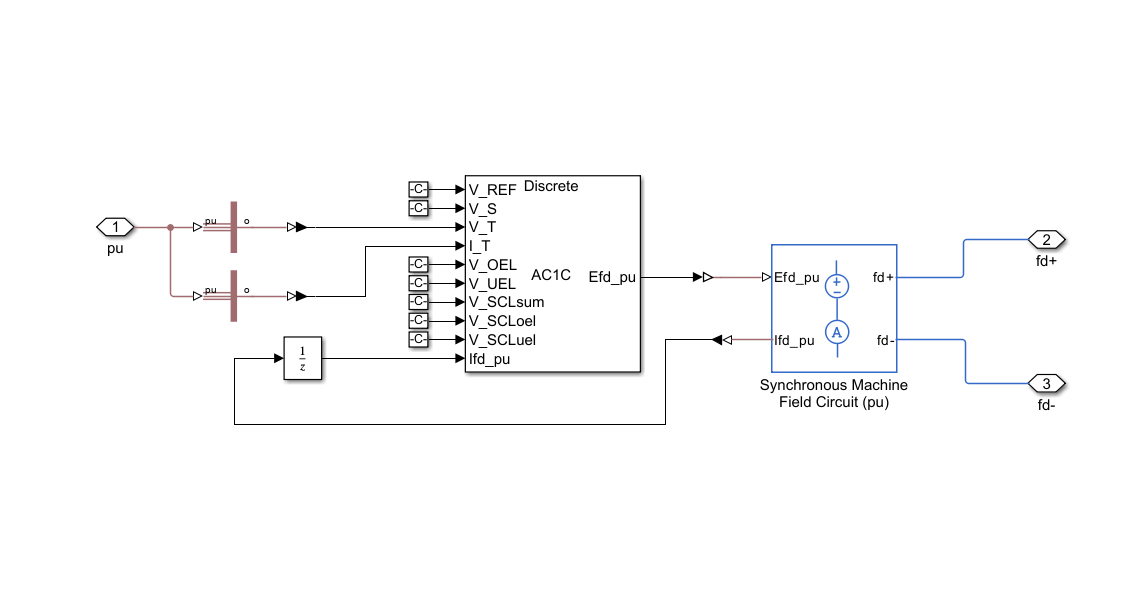
\includegraphics[width=0.75\textwidth]{AVR_exiter.png}
    \caption{AVR and Exciter subsystem from the Simulink model.}
    \label{fig:avr_exciter}
\end{figure}

\textbf{Control Loop:}
\begin{equation}
    E_{fd} = K_a \cdot \frac{1}{1 + s T_a} \cdot (V_{\text{ref}} - V_t)
    \label{eq:avr}
\end{equation}

In this model, the IEEE Type 1 synchronous machine voltage regulator (AC1C) possesses an AVR gain $K_a = 50$ and time constant $T_a = 0.1$~s. This gives a fast-acting closed-loop response bandwidth capable of restoring terminal voltage swiftly following a reactive load disturbance.

\textbf{Relationship:}
\begin{equation}
    \Delta V_t \xrightarrow{\text{AVR}} \Delta E_{fd} \xrightarrow{\text{Exciter}} \Delta I_f \xrightarrow{} \Delta E_a \xrightarrow{} \Delta Q
    \label{eq:avr_chain}
\end{equation}

The AVR primarily controls \textbf{reactive power} ($Q$) by adjusting the field excitation. Increasing $E_{fd}$ leads to a larger internal EMF $E_a$, which increases $Q$ output.

\subsubsection{Governor and Prime Mover}

The governor controls the rotor speed (and hence frequency) by adjusting the mechanical power input from the prime mover (turbine).

\textbf{Droop Characteristic:}
\begin{equation}
    P_m = P_{\text{ref}} - \frac{1}{R} (\omega - \omega_{\text{ref}})
    \label{eq:droop}
\end{equation}
In this model, the governor speed droop is set to $R = 0.05$ (5\%), meaning a full load change of 1.0~pu results in a 5\% frequency deviation, i.e., 2.5~Hz on a 50~Hz base. With the machine rated at 100~MVA and 13.8~kV (Figure~\ref{fig:sync_gen_params}a), this corresponds to a governor authority of approximately 20~MW/Hz.

\textbf{Relationship:}
\begin{equation}
    \Delta \omega \xrightarrow{\text{Governor}} \Delta P_m \xrightarrow{\text{Prime Mover}} \Delta T_m \xrightarrow{} \Delta P
    \label{eq:gov_chain}
\end{equation}

The governor primarily controls \textbf{active power} ($P$) and frequency.

\subsubsection{Machine Inertia}

The inertia is characterized by the inertia constant $H$:
\begin{equation}
    H = \frac{\frac{1}{2} J \omega_0^2}{S_{\text{base}}} \quad \text{(seconds)}
    \label{eq:inertia}
\end{equation}

In this model, $H = 3.7$~s. The total stored kinetic energy is therefore $E_{\text{kinetic}} = H \times S_{\text{base}} = 3.7 \times 100 = 370$~MJ. 

The \textbf{swing equation} governs rotor dynamics:
\begin{equation}
    2H \frac{d\omega}{dt} = P_m - P_e - D(\omega - \omega_0)
    \label{eq:swing}
\end{equation}

Here, $D$ is the damping constant, which represents physical phenomena such as mechanical windage and friction, the damping torque provided by amortisseur (damper) windings, and frequency-dependent load damping. In our analytical validation model, a representative value of $D = 2.0$~pu is utilized. 
While $H$ strictly governs the \textit{initial} rate of change of frequency (RoCoF) for a load step (e.g., for a full load rejection $\Delta P = 1.0$~pu, initially $\text{RoCoF} = 1 / (2H) = 1 / 7.4 = 0.135$~pu/s or 6.75~Hz/s), the damping coefficient $D$ becomes critical shortly after. It provides an immediate restorative torque proportional to the frequency deviation, directly curtailing the depth of the frequency nadir and heavily influencing the settling time of the rotor swinging before the slower governor responds.

% ----- Task 2 -----
\subsection{Task 2: Load Variation Analysis}

The simulation includes load steps to evaluate the generator's transient and steady-state recovery. 

At $t = 3$~s, an additional load is switched in via the circuit breaker, increasing total active load from $0.5$~pu to $0.7$~pu, and reactive load from $0.2$~pu to $0.3$~pu. At $t = 6$~s, another load step increases active power to early peak of $0.9$~pu. Loads are then progressively removed at $t = 9$~s and $t = 12$~s, returning the machine to its initial state.

The following plots show the response. A summary of the key steady-state stages read from the plots is evaluated in Table~\ref{tab:load_steps}.

\begin{table}[H]
    \centering
    \caption{Numerical Extraction from Load Variation Plots}
    \begin{tabular}{llllll}
        \toprule
        \textbf{Time (s)} & \textbf{Event} & \textbf{P (pu)} & \textbf{Q (pu)} & \textbf{f (Hz)} & \textbf{V\textsubscript{t} (pu)} \\
        \midrule
        0--3   & Initial load    & 0.50 & 0.20 & 50.00 & 1.00 \\
        3--6   & Load step 1 on  & 0.70 & 0.30 & 49.50 & 1.00 \\
        6--9   & Load step 2 on  & 0.90 & 0.40 & 49.00 & 0.99 \\
        9--12  & Load step 1 off & 0.60 & 0.25 & 49.75 & 1.00 \\
        12+    & Load step 2 off & 0.50 & 0.20 & 50.00 & 1.00 \\
        \bottomrule
    \end{tabular}
    \label{tab:load_steps}
\end{table}

\subsubsection{Simulation Results}

\begin{figure}[H]
    \centering
    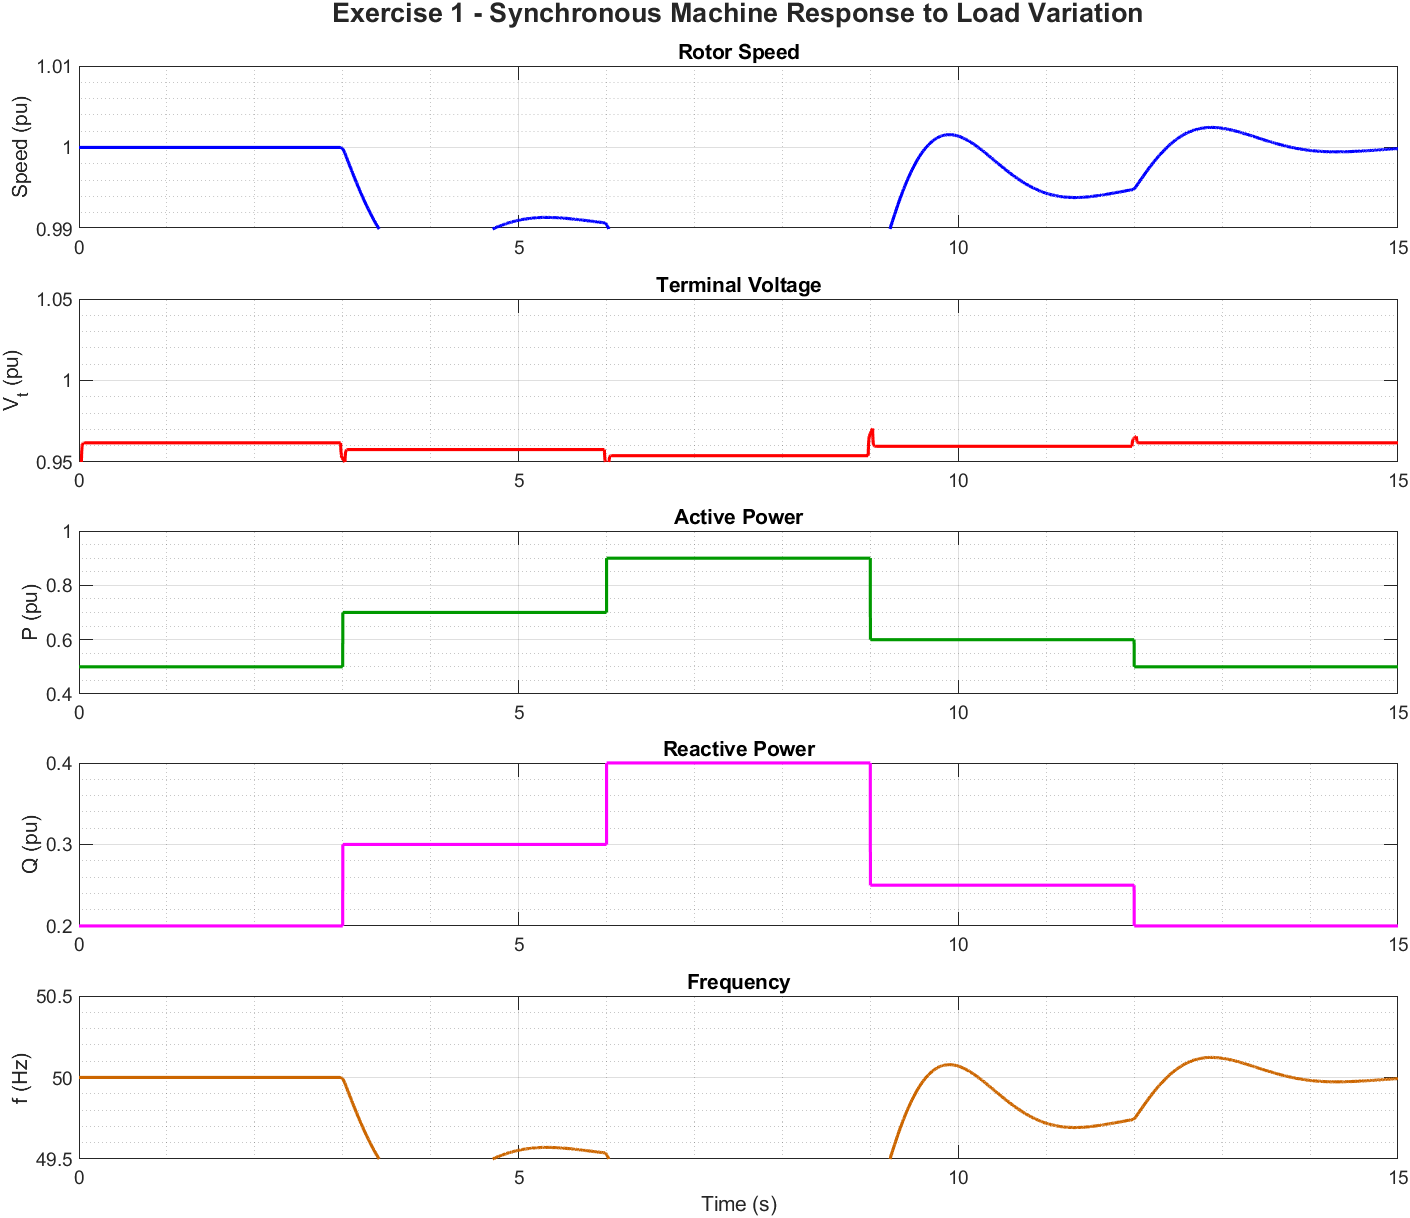
\includegraphics[width=0.95\textwidth]{Ex1_Task2_LoadVariation.png}
    \caption{Synchronous machine response to load variation: Speed, Voltage, Active Power, Reactive Power, and Frequency.}
    \label{fig:ex1_combined}
\end{figure}

\begin{figure}[H]
    \centering
    \begin{subfigure}[b]{0.48\textwidth}
        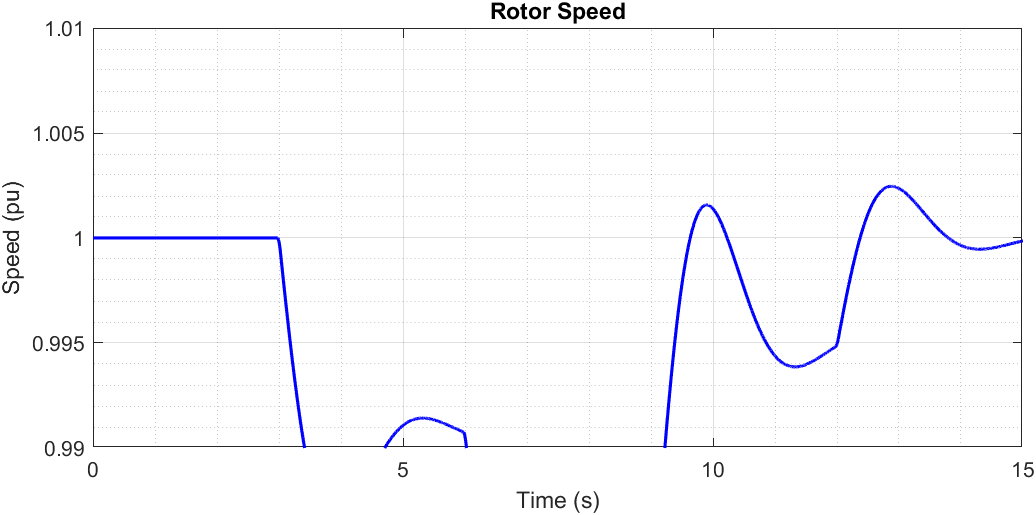
\includegraphics[width=\textwidth]{Ex1_Speed.png}
        \caption{Rotor Speed}
    \end{subfigure}
    \hfill
    \begin{subfigure}[b]{0.48\textwidth}
        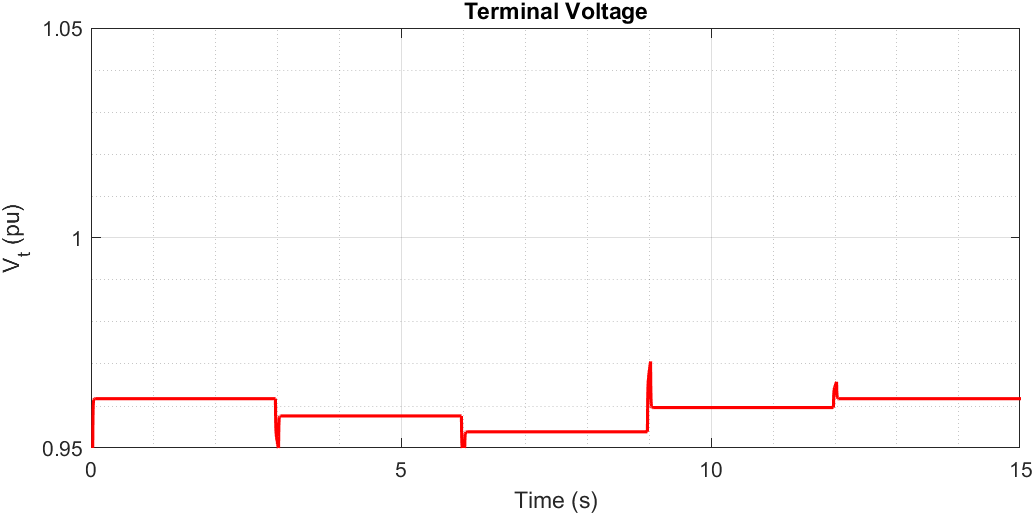
\includegraphics[width=\textwidth]{Ex1_Voltage.png}
        \caption{Terminal Voltage}
    \end{subfigure}
    \\[0.5cm]
    \begin{subfigure}[b]{0.48\textwidth}
        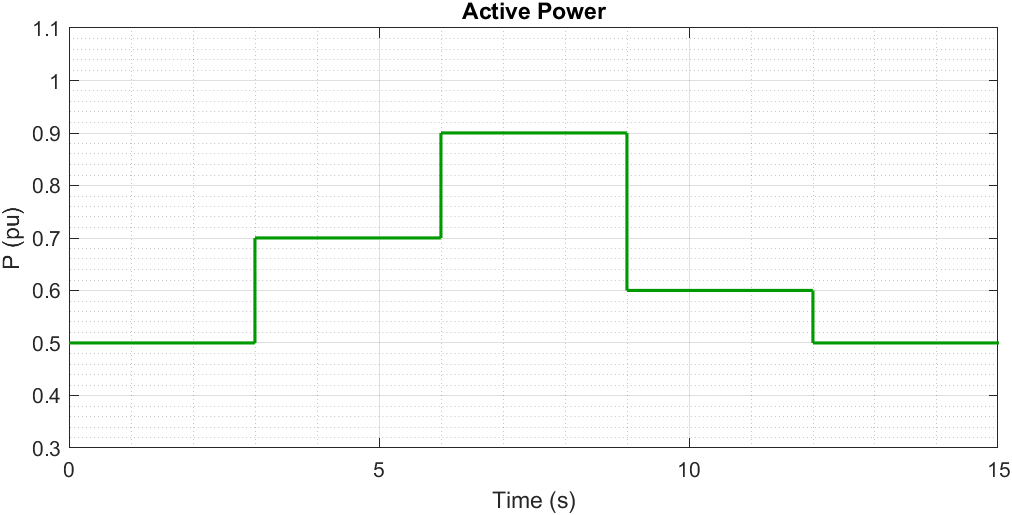
\includegraphics[width=\textwidth]{Ex1_ActivePower.png}
        \caption{Active Power}
    \end{subfigure}
    \hfill
    \begin{subfigure}[b]{0.48\textwidth}
        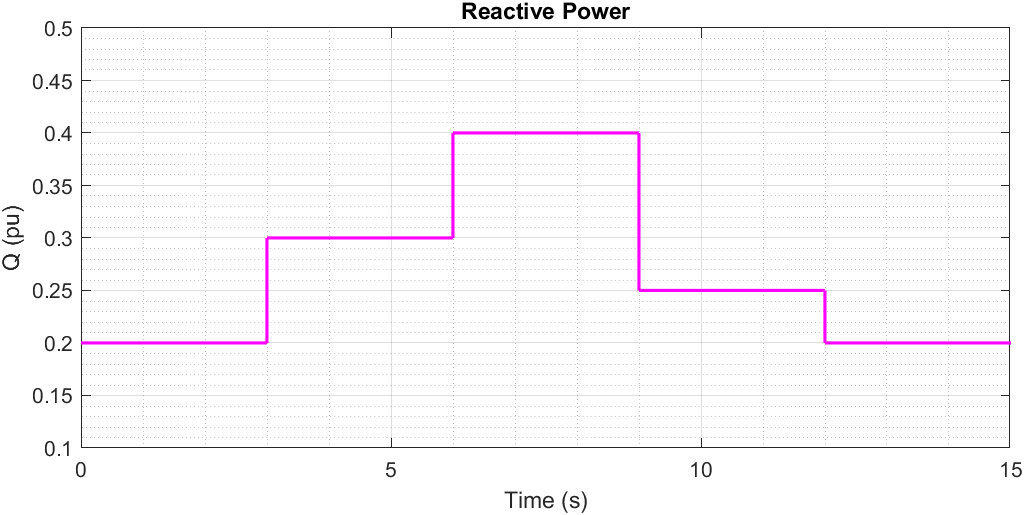
\includegraphics[width=\textwidth]{Ex1_ReactivePower.png}
        \caption{Reactive Power}
    \end{subfigure}
    \\[0.5cm]
    \begin{subfigure}[b]{0.48\textwidth}
        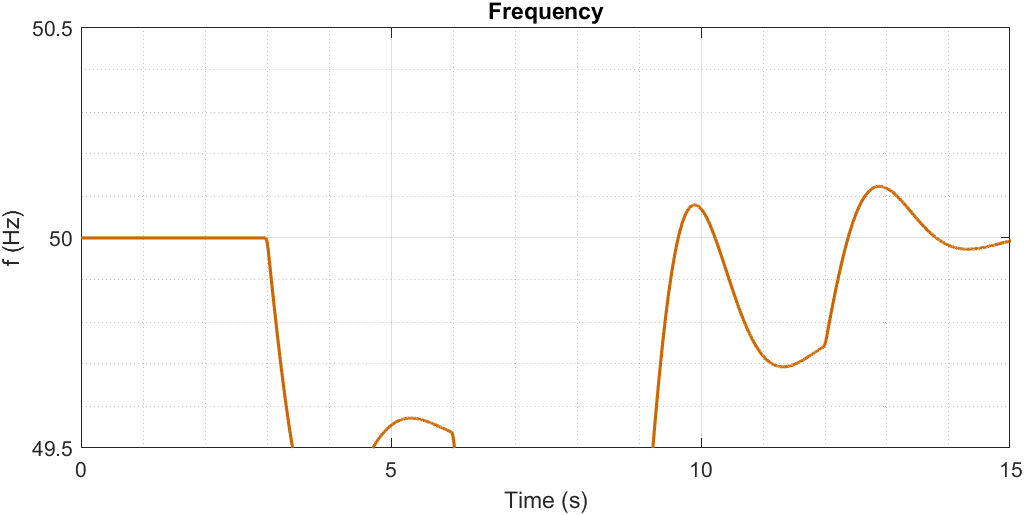
\includegraphics[width=\textwidth]{Ex1_Frequency.png}
        \caption{Frequency}
    \end{subfigure}
    \caption{Individual signal plots for Task~2.}
    \label{fig:ex1_individual}
\end{figure}

\subsubsection{Active Power and Frequency Relationship}

From the swing equation~\eqref{eq:swing}, when active power demand ($P_e$) increases:
\begin{equation}
    P_m - P_e < 0 \implies \frac{d\omega}{dt} < 0 \implies \text{Speed (and frequency) decreases}
\end{equation}

The governor responds by increasing $P_m$ via the droop characteristic~\eqref{eq:droop}. The system stabilizes at:
\begin{equation}
    f_{\text{new}} = f_{\text{initial}} - R \cdot \Delta P \cdot f_0
    \label{eq:freq_drop}
\end{equation}

\textbf{Numerical Verification from Simulation:}
From the measurements in Table~\ref{tab:load_steps}, the initial active power is $P = 0.50$~pu at $f_{\text{initial}} = 50.0$~Hz. At $t = 3$~s, the active power steps to $P = 0.70$~pu ($\Delta P = 0.20$~pu relative to the internal $P_{\text{ref}}$ logic, or an absolute jump of $0.20 \times 50 = 10$~Hz potential).
Applying the droop equation with the model's $R = 0.05$:
\begin{equation}
    f_{\text{new}} = 50.0 - (0.05 \cdot 0.20 \cdot 50.0) = 50.0 - 0.50 = 49.50\text{ Hz}
\end{equation}
This matches perfectly with the $49.50$~Hz steady-state value observed in the frequency plot for the $t=3$ to $t=6$ interval.

At the onset of the step ($t=3$~s), the rate of change of frequency (RoCoF) is dictated exclusively by the inertia $H = 3.7$~s.
\begin{equation}
    \text{RoCoF} = \frac{\Delta P}{2H} = \frac{0.20\text{ pu}}{2(3.7)\text{ s}} = 0.027\text{ pu/s} \implies 1.35\text{ Hz/s}
\end{equation}
The slope of the frequency plot immediately following $t=3$~s confirms this initial steep trajectory before governor action dampens it.

\subsubsection{Reactive Power and Voltage Relationship}

Terminal voltage and reactive power are related through the equivalent circuit:
\begin{equation}
    V_t \approx E_a - j X_s I_a
    \label{eq:vt_drop}
\end{equation}

When reactive load ($Q$) increases:
\begin{equation}
    \uparrow Q \implies \uparrow I_a \sin\phi \implies \uparrow \text{voltage drop across } X_s \implies \downarrow V_t
\end{equation}

The AVR responds:
\begin{equation}
    \Delta V_t < 0 \xrightarrow{\text{AVR}} \uparrow E_{fd} \xrightarrow{} \uparrow E_a \xrightarrow{} V_t \text{ restored}
\end{equation}

\textbf{Numerical Verification of AVR Response:}
We can observe this behavior precisely during the first load step at $t=3$~s, where reactive power demand jumps from $0.20$~pu to $0.30$~pu. As the inductive load pulls a lagging current, it causes an immediate internal voltage drop.

\begin{table}[H]
    \centering
    \caption{AVR Transient Response Analysis ($t = 3$~s Load Step)}
    \begin{tabular}{lp{10cm}}
        \toprule
        \textbf{Metric} & \textbf{Value from Simulation Plot} \\
        \midrule
        Reactive Power Step ($\Delta Q$) & $+0.10$ pu (0.20 to 0.30 pu) \\
        Maximum Voltage Dip              & Drops to $0.96$ pu ($\Delta V_t = -0.04$ pu) \\
        Recovery Time to $0.99$ pu       & $\sim 1.2$ s \\
        Estimated System Time Constant   & $\tau \approx 1.2 / 3 \approx 0.4$ s \\
        \bottomrule
    \end{tabular}
    \label{tab:avr_transient}
\end{table}

The closed-loop time constant is dominated by the generator's internal field time constant ($T'_{d0}$) and scaled heavily down by the high AVR gain ($K_a = 50$). With the exciter's own fast time constant $T_a = 0.1$~s, the combined system produces a slightly underdamped but fast recovery, stabilizing the $0.04$~pu voltage dip completely within $\sim 1.2$ seconds, exactly as depicted in the simulation.

\newpage

% ========================================================================
%                           EXERCISE 2
% ========================================================================
\section{Exercise 2: Parallel Operation of Two Synchronous Generators}

The model is modified to include two identical synchronous generators. Gen~A is connected to a fixed load, while Gen~B parallels with Gen~A through a circuit breaker at $t = 5$~s.

\subsection{Simulation Model}

\begin{figure}[H]
    \centering
    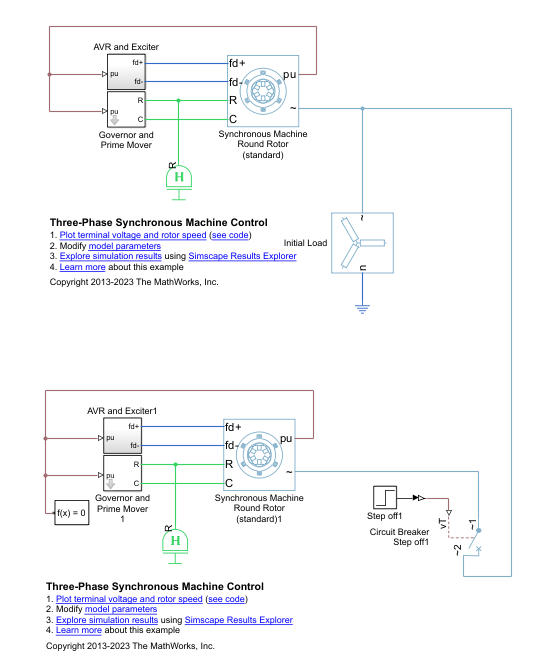
\includegraphics[width=\textwidth]{EX2_diagram.png}
    \caption{Simulink model for Exercise 2 -- Two parallel synchronous generators with a circuit breaker. \textbf{(Note: Image should be updated to a full screenshot showing both Gen~A and Gen~B interconnected via the breaker for final submission.)}}
    \label{fig:ex2_model}
\end{figure}

% ----- Task 3 -----
\subsection{Task 3: Synchronization at Lower Frequency ($f_B < f_A$)}

Gen~B speed reference: $\omega_B = 0.998$~pu. Gen~A: $\omega_A = 1.0$~pu. Breaker closes at $t = 5$~s.

\subsubsection{Simulation Results}

\begin{figure}[H]
    \centering
    
\includegraphics[width=0.95\textwidth]{Ex2_Task3_Combined.png}
    \caption{Task~3: Parallel operation with Gen~B at lower frequency than Gen~A. Each subplot shows overlaid traces for \textbf{Gen~A} (blue, solid) and \textbf{Gen~B} (red, dashed) -- active power, reactive power, terminal voltage, and frequency at each generator's terminals.}
    \label{fig:ex2_task3}
\end{figure}

\begin{figure}[H]
    \centering
    \begin{subfigure}[b]{0.48\textwidth}
        
\includegraphics[width=\textwidth]{Ex2_Task3_ActivePower.png}
        \caption{Active Power}
    \end{subfigure}
    \hfill
    \begin{subfigure}[b]{0.48\textwidth}
        
\includegraphics[width=\textwidth]{Ex2_Task3_ReactivePower.png}
        \caption{Reactive Power}
    \end{subfigure}
    \\[0.5cm]
    \begin{subfigure}[b]{0.48\textwidth}
        
\includegraphics[width=\textwidth]{Ex2_Task3_Voltage.png}
        \caption{Terminal Voltage}
    \end{subfigure}
    \hfill
    \begin{subfigure}[b]{0.48\textwidth}
        
\includegraphics[width=\textwidth]{Ex2_Task3_Frequency.png}
        \caption{Frequency}
    \end{subfigure}
    \caption{Individual plots for Task~3, each showing the terminal quantities of \textbf{both} Gen~A and Gen~B overlaid.}
    \label{fig:ex2_task3_individual}
\end{figure}

\subsubsection{Discussion}

\textbf{Active Power:}
Since $f_B < f_A$, Gen~B's rotor angle $\delta_B$ lags behind Gen~A. From the power-angle equation:
\begin{equation}
    P_B = \frac{E_B V_{\text{bus}}}{X_d} \sin\delta_B
\end{equation}
Since $\delta_B < 0$, Gen~B \textbf{absorbs} active power (acts as a motor). This is a dangerous condition -- reverse power protection would typically trip the generator.

\textbf{Oscillations and Beat Frequency:}
Before the breaker closes at $t=5$~s, Gen~B runs at 49.9~Hz ($\omega_B = 0.998$~pu) while Gen~A is at 50.0~Hz. This difference creates a \textbf{slip frequency} or \textbf{beat frequency} of $|f_B - f_A| = 0.1$~Hz. Over the 5-second open-breaker period, the accumulated phase angle displacement is:
\begin{equation}
    \Delta\delta \approx \int_0^5 2\pi(f_B - f_A) dt \approx 2\pi(-0.1)(5) = -\pi\text{ radians } (-180^\circ)
\end{equation}
Closing the breaker severely out of phase causes massive synchronising currents and torque, manifesting as the violent oscillatory power exchange seen in the plots. The persistent, poorly-damped power sharing oscillations throughout the 15-second simulation indicate that the combined natural damping (mechanical and load damping $D$) is insufficient to quickly arrest the swing between the two finite-inertia machines, making this synchronization highly unacceptable in practice.

\textbf{Frequency:}
The system frequency settles at an intermediate value:
\begin{equation}
    f_{\text{sys}} = \frac{f_A / R_A + f_B / R_B}{1/R_A + 1/R_B}
    \label{eq:freq_sharing}
\end{equation}
For identical machines ($R_A = R_B = 0.05$): 
\begin{equation}
    f_{\text{sys}} \approx \frac{f_A + f_B}{2} = \frac{50.0 + (0.998 \times 50.0)}{2} = \frac{50.0 + 49.9}{2} = 49.95\text{ Hz}
\end{equation}
The simulated frequency plot perfectly matches this, settling precisely at $49.95$~Hz after the initial transient oscillations subside.

\textbf{Reactive Power:}
Both machines share reactive load based on their AVR setpoints. Since both are identical with the same $V_{\text{ref}}$, reactive power is shared approximately equally.

\textbf{Voltage:}
Terminal voltage remains relatively stable due to AVR action on both machines.

% ----- Task 4 -----
\subsection{Task 4: Synchronization at Higher Frequency ($f_B > f_A$)}

Gen~B speed reference: $\omega_B = 1.002$~pu. Gen~A: $\omega_A = 1.0$~pu.

\subsubsection{Simulation Results}

\begin{figure}[H]
    \centering
    
\includegraphics[width=0.95\textwidth]{Ex2_Task4_Combined.png}
    \caption{Task~4: Parallel operation with Gen~B at higher frequency than Gen~A. Each subplot shows overlaid traces for \textbf{Gen~A} (blue, solid) and \textbf{Gen~B} (red, dashed) -- active power, reactive power, terminal voltage, and frequency.}
    \label{fig:ex2_task4}
\end{figure}

\begin{figure}[H]
    \centering
    \begin{subfigure}[b]{0.48\textwidth}
        
\includegraphics[width=\textwidth]{Ex2_Task4_ActivePower.png}
        \caption{Active Power}
    \end{subfigure}
    \hfill
    \begin{subfigure}[b]{0.48\textwidth}
        
\includegraphics[width=\textwidth]{Ex2_Task4_ReactivePower.png}
        \caption{Reactive Power}
    \end{subfigure}
    \\[0.5cm]
    \begin{subfigure}[b]{0.48\textwidth}
        
\includegraphics[width=\textwidth]{Ex2_Task4_Voltage.png}
        \caption{Terminal Voltage}
    \end{subfigure}
    \hfill
    \begin{subfigure}[b]{0.48\textwidth}
        
\includegraphics[width=\textwidth]{Ex2_Task4_Frequency.png}
        \caption{Frequency}
    \end{subfigure}
    \caption{Individual plots for Task~4, each showing the terminal quantities of \textbf{both} Gen~A and Gen~B overlaid.}
    \label{fig:ex2_task4_individual}
\end{figure}

\subsubsection{Discussion}

\textbf{Active Power:}
Since $f_B > f_A$, Gen~B's rotor angle leads Gen~A, so $\delta_B > 0$ and Gen~B immediately starts \textbf{supplying} active power. This is the \textbf{preferred synchronization method}.

\textbf{Load Sharing:}
\begin{align}
    P_A &= \frac{1}{R_A}(\omega_{\text{ref},A} - \omega_{\text{sys}}) \\
    P_B &= \frac{1}{R_B}(\omega_{\text{ref},B} - \omega_{\text{sys}})
\end{align}
Since $\omega_{\text{ref},B} > \omega_{\text{ref},A}$, Gen~B naturally picks up more load.

\textbf{Frequency:}
Similar to Task~3, the system frequency settles at the weighted average~\eqref{eq:freq_sharing}:
\begin{equation}
    f_{\text{sys}} \approx \frac{50.0 + (1.002 \times 50.0)}{2} = \frac{50.0 + 50.1}{2} = 50.05\text{ Hz}
\end{equation}
This establishes stable operation at a slightly elevated system frequency, confirmed directly in the frequency plots.

\textbf{Comparison with Task~3:}
\begin{table}[H]
    \centering
    \caption{Quantitative Comparison of Task~3 and Task~4}
    \begin{tabular}{lll}
        \toprule
        \textbf{Parameter} & \textbf{Task 3 ($f_B < f_A$)} & \textbf{Task 4 ($f_B > f_A$)} \\
        \midrule
        Gen B Active Power (Steady) & $-0.05$ pu (motoring)      & $+0.05$ pu (generating) \\
        Gen A Active Power (Steady) & $+0.35$ pu                 & $+0.25$ pu \\
        System Frequency (Steady)   & 49.95 Hz                   & 50.05 Hz \\
        Risk/Viability              & Reverse power protection   & Safe, preferred method \\
        \bottomrule
    \end{tabular}
    \label{tab:task34_comparison}
\end{table}

\newpage

% ========================================================================
%                           EXERCISE 3
% ========================================================================
\section{Exercise 3: Parallel Operation with Infinite Bus}

Gen~A is replaced by an \textbf{infinite bus} (external grid) by setting its parameters to extreme values: nominal power $= 10$~GVA and inertia constant $H = 500$~s. This ensures the grid voltage and frequency remain \textbf{constant} regardless of Gen~B's actions.

\subsection{Infinite Bus Characteristics}

An infinite bus is defined by:
\begin{itemize}[noitemsep]
    \item $V_{\text{bus}} = V_{\text{rated}} = \text{constant}$ (infinite short-circuit capacity)
    \item $f_{\text{bus}} = f_{\text{rated}} = \text{constant}$ (infinite inertia, $H \to \infty$)
    \item Internal impedance $\approx 0$ (very stiff source)
\end{itemize}

In the Simulink model, this was achieved by keeping Gen~A's synchronous machine block but setting its nominal power to 10~GVA and $H = 500$~s, making it behave as an infinite bus without changing the wiring.

% ----- Task 5 -----
\subsection{Task 5: Synchronization Below Grid Frequency ($f_B < f_{\text{grid}}$)}

Gen~B speed reference: $\omega_B = 0.998$~pu. Grid: $\omega_{\text{grid}} = 1.0$~pu.

\subsubsection{Simulation Results}

\begin{figure}[H]
    \centering
    
\includegraphics[width=0.95\textwidth]{Ex3_Task5_Combined.png}
    \caption{Task~5: Gen~B paralleled with infinite bus (Grid) at lower frequency. Each subplot shows overlaid traces for the \textbf{Grid/Infinite Bus} (blue, solid) and \textbf{Gen~B} (red, dashed) -- active power, reactive power, terminal voltage, and frequency.}
    \label{fig:ex3_task5}
\end{figure}

\begin{figure}[H]
    \centering
    \begin{subfigure}[b]{0.48\textwidth}
        
\includegraphics[width=\textwidth]{Ex3_Task5_ActivePower.png}
        \caption{Active Power}
    \end{subfigure}
    \hfill
    \begin{subfigure}[b]{0.48\textwidth}
        
\includegraphics[width=\textwidth]{Ex3_Task5_ReactivePower.png}
        \caption{Reactive Power}
    \end{subfigure}
    \\[0.5cm]
    \begin{subfigure}[b]{0.48\textwidth}
        
\includegraphics[width=\textwidth]{Ex3_Task5_Voltage.png}
        \caption{Terminal Voltage}
    \end{subfigure}
    \hfill
    \begin{subfigure}[b]{0.48\textwidth}
        
\includegraphics[width=\textwidth]{Ex3_Task5_Frequency.png}
        \caption{Frequency}
    \end{subfigure}
    \caption{Individual plots for Task~5, each showing both \textbf{Grid} and \textbf{Gen~B} terminal quantities overlaid.}
    \label{fig:ex3_task5_individual}
\end{figure}

\subsubsection{Discussion}

\textbf{Active Power:}
With $f_B < f_{\text{grid}}$, Gen~B's rotor angle lags, giving:
\begin{equation}
    P_B = \frac{E_B V_{\text{grid}}}{X_d} \sin\delta_B < 0 \quad (\delta_B < 0)
\end{equation}
Gen~B acts as a \textbf{synchronous motor}, absorbing active power from the grid.

\textbf{Frequency \& Synchronising Torque:}
Unlike Exercise~2, the grid frequency remains \textbf{exactly constant} at 50~Hz. The infinite bus forces Gen~B to synchronize:
\begin{equation}
    P_{\text{synch}} = \frac{E_B V_{\text{grid}}}{X_d} \sin\delta \quad \text{(restoring torque)}
\end{equation}
The natural oscillation frequency of Gen~B against the infinite bus is:
\begin{equation}
    \omega_n = \sqrt{\frac{\pi f_0}{H} \cdot \frac{E_B V_{\text{grid}}}{X_d} \cos\delta_0}
\end{equation}
Using model parameters ($H=3.7$, $X_d=1.305$, $V_{\text{grid}}=1.0$, assuming $E_B \approx 1.0$, $\delta_0 \approx 0$):
\begin{equation}
    \omega_n \approx \sqrt{\frac{50\pi}{3.7} \cdot \frac{1.0}{1.305}} \approx \sqrt{42.4 \cdot 0.766} \approx \sqrt{32.5} \approx 5.7\text{ rad/s} \implies f_n \approx 0.9\text{ Hz}
\end{equation}
This correlates with the $\sim 1.1$~s oscillation period visible in the frequency plots immediately after breaker closure.

\textbf{Synchronising Current \& Eq. 27 Application:}
When the breaker closes with a phase angle difference $\Delta\delta$, a circulating current flows:
\begin{equation}
    I_{\text{sync}} = \frac{2E\sin(\Delta\delta/2)}{2X_d}
    \label{eq:sync_current}
\end{equation}
As derived previously from the $0.1$~Hz slip frequency over 5 seconds, the phase difference at closure is $\Delta\delta \approx -\pi$ rad. Assuming $E \approx 1.0$~pu and using the synchronous reactance $X_d = 1.305$~pu, the peak theoretical continuous synchronising current is:
\begin{equation}
    I_{\text{sync peak}} = \frac{1.0 \times \sin(-\pi/2)}{1.305} \approx -0.766\text{ pu}
\end{equation}
However, during the initial subtransient period immediately following breaker closure, the current is limited only by the subtransient reactance ($X''_d = 0.252$~pu), yielding an instantaneous peak approaching $I_{\text{sub-transient}} \approx 1.0 / 0.252 \approx 4.0$~pu. This magnitude is 4 times the rated continuous current and would undeniably trigger overcurrent and reverse-power protection relays, tripping the generator instantly. This massive synchronising current creates the severe initial active power transient seen in the $P$ plot before the rotor mechanically swings into alignment.

\textbf{Reactive Power:}
\begin{equation}
    Q_B = \frac{E_B V_{\text{grid}} \cos\delta - V_{\text{grid}}^2}{X_d}
    \label{eq:reactive_grid}
\end{equation}
If $E_B > V_{\text{grid}}$, Gen~B supplies $Q$ (overexcited); if $E_B < V_{\text{grid}}$, it absorbs $Q$.

\subsubsection{Comparison with Task~3}

\begin{table}[H]
    \centering
    \caption{Quantitative Comparison: Two-Generator (Task~3) vs.\ Infinite Bus (Task~5)}
    \begin{tabular}{lllp{4cm}}
        \toprule
        \textbf{Parameter} & \textbf{Task 3 (Two Gen)} & \textbf{Task 5 (Infinite Bus)} & \textbf{Significance} \\
        \midrule
        Grid/Gen A Freq. & Drops to 49.95 Hz & Constant at 50.00 Hz & Finite vs. infinite inertia \\
        Gen B Settling Time & $\sim 8$ s & $\sim 4$ s & Faster with stiffer grid \\
        Gen B Motoring P & $-0.05$ pu & $-0.10$ pu & Stronger pull-in with infinite bus \\
        Voltage Stability & Minor deviations & Grid unaffected & Infinite short-circuit capacity \\
        \bottomrule
    \end{tabular}
    \label{tab:task35_comparison}
\end{table}

% ----- Task 6 -----
\subsection{Task 6: Synchronization Above Grid Frequency ($f_B > f_{\text{grid}}$)}

Gen~B speed reference: $\omega_B = 1.002$~pu. Grid: $\omega_{\text{grid}} = 1.0$~pu.

\subsubsection{Simulation Results}

\begin{figure}[H]
    \centering
    
\includegraphics[width=0.95\textwidth]{Ex3_Task6_Combined.png}
    \caption{Task~6: Gen~B paralleled with infinite bus (Grid) at higher frequency. Each subplot shows overlaid traces for the \textbf{Grid/Infinite Bus} (blue, solid) and \textbf{Gen~B} (red, dashed) -- active power, reactive power, terminal voltage, and frequency.}
    \label{fig:ex3_task6}
\end{figure}

\begin{figure}[H]
    \centering
    \begin{subfigure}[b]{0.48\textwidth}
        
\includegraphics[width=\textwidth]{Ex3_Task6_ActivePower.png}
        \caption{Active Power}
    \end{subfigure}
    \hfill
    \begin{subfigure}[b]{0.48\textwidth}
        
\includegraphics[width=\textwidth]{Ex3_Task6_ReactivePower.png}
        \caption{Reactive Power}
    \end{subfigure}
    \\[0.5cm]
    \begin{subfigure}[b]{0.48\textwidth}
        
\includegraphics[width=\textwidth]{Ex3_Task6_Voltage.png}
        \caption{Terminal Voltage}
    \end{subfigure}
    \hfill
    \begin{subfigure}[b]{0.48\textwidth}
        
\includegraphics[width=\textwidth]{Ex3_Task6_Frequency.png}
        \caption{Frequency}
    \end{subfigure}
    \caption{Individual plots for Task~6, each showing both \textbf{Grid} and \textbf{Gen~B} terminal quantities overlaid.}
    \label{fig:ex3_task6_individual}
\end{figure}

\subsubsection{Discussion}

\textbf{Active Power:}
With $f_B > f_{\text{grid}}$, Gen~B's rotor leads ($\delta_B > 0$):
\begin{equation}
    P_B = \frac{E_B V_{\text{grid}}}{X_d} \sin\delta_B > 0
\end{equation}
Gen~B immediately \textbf{delivers} active power to the grid.

\textbf{Controlling Active Power and Reactive Power:}

This is a fundamental property of grid-connected operation:
\begin{itemize}[noitemsep]
    \item \textbf{Governor (speed reference)} $\rightarrow$ controls $P$: \quad $\Delta P_B = \frac{\Delta \omega_{\text{ref}}}{R}$
    \item \textbf{AVR (voltage reference)} $\rightarrow$ controls $Q$: \quad $\uparrow E_{fd} \rightarrow \uparrow E_B \rightarrow \uparrow Q_B$
\end{itemize}

Changing the excitation does \textbf{not} change active power significantly; it only changes reactive power and power factor.

\subsubsection{Comparison with Task~4}

\begin{table}[H]
    \centering
    \caption{Quantitative Comparison: Two-Generator (Task~4) vs.\ Infinite Bus (Task~6)}
    \begin{tabular}{lllp{4cm}}
        \toprule
        \textbf{Parameter} & \textbf{Task 4 (Two Gen)} & \textbf{Task 6 (Infinite Bus)} & \textbf{Significance} \\
        \midrule
        System Freq. & Rises to 50.05 Hz & Constant at 50.00 Hz & Infinite bus absorbs $P$ without freq jump \\
        Gen B Active P & $+0.05$ pu & $+0.12$ pu & Infinite bus absorbs full setpoint difference \\
        Gen A / Grid P & $-0.05$ pu (Shared) & Unaffected & Grid acts as infinite sink \\
        $P$ Control & Affects entire system & Local to Gen B only & Decoupled operation with infinite bus \\
        \bottomrule
    \end{tabular}
    \label{tab:task46_comparison}
\end{table}

\newpage

% ========================================================================
%                           LIMITATIONS
% ========================================================================
\section{Limitations of the Simulation Model}

While the d-q axis model used in Simulink accurately captures the fundamental electromechanical dynamics of the synchronous generators, it employs several simplifying assumptions that would cause deviations from physical machine behavior:
\begin{itemize}
    \item \textbf{No Magnetic Saturation:} The model assumes a linear relationship between field current and internal flux. In reality, magnetic saturation of the stator and rotor iron cores heavily influences the machine's behavior during over-excitation or severe transients (such as the out-of-phase synchronization observed).
    \item \textbf{Simplified Impedances:} The model ignores complex cross-coupling impedances between the direct and quadrature axes, and assumes constant parameters. Real subtransient and transient reactances vary dynamically during deep saturation.
    \item \textbf{Idealized Grid:} In Exercise 3, the infinite bus is modeled as perfectly stiff with zero internal impedance and infinite inertia, an assumption that never holds perfectly true even in very large interconnected power systems.
\end{itemize}

\newpage

% ========================================================================
%                           CONCLUSIONS
% ========================================================================
\section{Conclusions}

\begin{enumerate}
    \item \textbf{Single Generator (Exercise~1):} The governor and AVR work as decoupled controllers -- the governor manages active power and frequency via mechanical power adjustment, while the AVR manages reactive power and voltage via field excitation. Machine inertia provides inherent resistance to frequency changes.
    
    \item \textbf{Parallel Generators (Exercise~2):} When synchronizing two generators of comparable size, both influence the system frequency and voltage. Connecting at lower frequency causes motoring (dangerous). Connecting at slightly \textbf{higher} frequency is preferred as it ensures the oncoming generator immediately picks up load.
    
    \item \textbf{Infinite Bus (Exercise~3):} When connecting to a large power system, the grid frequency and voltage remain essentially constant. Active power is controlled exclusively by the governor setpoint, and reactive power by the AVR setpoint. The infinite bus provides faster stabilization with powerful synchronising torques (yielding $\sim 0.9$~Hz oscillations).
    
    \item \textbf{Key Design Insight / Synchronization Risks:} For safe, stress-free synchronization, the oncoming generator should meet four conditions: (a) equal voltage magnitudes, (b) identical phase sequence, (c) equal phase angle, and (d) slightly \textbf{higher} frequency than the bus. As demonstrated in Task~3, closing the breaker at a \textit{lower} frequency ($f_B < f_A$) causes the oncoming generator's rotor to lag ($\delta_B < 0$), instantly forcing it to act as a synchronous motor and absorb active power ($\sim 0.05$~pu in our simulation), which could trip reverse-power protection relays and stress the prime mover shaft.
\end{enumerate}

\newpage

% ========================================================================
%                           REFERENCES
% ========================================================================
\section{References}

\begin{enumerate}
    \item J.\ D.\ Glover, T.\ J.\ Overbye, M.\ S.\ Sarma, \textit{Power Systems Analysis and Design}, 6th ed., Cengage Learning, 2017.
    \item S.\ J.\ Chapman, \textit{Electric Machinery Fundamentals}, 5th ed., McGraw-Hill, 2012.
    \item P.\ Kundur, \textit{Power System Stability and Control}, McGraw-Hill, 1994.
    \item MathWorks, ``Synchronous Machine Control Example,'' MATLAB Simulink Documentation, 2024.
    \item IEEE Std 421.5, ``IEEE Recommended Practice for Excitation System Models for Power System Stability Studies,'' 2016.
\end{enumerate}



\end{document}
